\documentclass[12pt]{article}
 
\usepackage[utf8]{inputenc}
\usepackage[T1]{fontenc}
\usepackage[french]{babel}
\usepackage{mathtools, bm}
\usepackage{amssymb, bm}
\usepackage{stmaryrd} 
\usepackage{enumitem}
\usepackage{array}
\usepackage{layout}
\usepackage{pslatex}
\usepackage{pstricks-add}
\usepackage{lmodern}
\usepackage{listings}
\usepackage{color}
\usepackage[pdfborder={0 0 0}]{hyperref}
\usepackage[babel=true]{csquotes}
\usepackage{amsthm}
\usepackage{thmtools, varioref}
\declaretheorem[title = Theorem, style=plain]{theo}
\newtheorem{plain}{Proposition}[section]
\usepackage{lmodern}
\usepackage{tikz}
\usepackage{setspace}
\usepackage{mathrsfs} % jolies cursives (mathscr)

% marge
\newcommand{\marge}[1]{\usepackage[top=#1,bottom=#1+1cm,left=#1,right=#1]{geometry}}
\newcommand{\smarge}[2]{\usepackage[top=#1,bottom=#1+1cm,left=#1-#2,right=#1]{geometry}}
\smarge{2.5cm}{0.6cm}
%\usepackage[top=2cm,bottom=2cm,left=2cm,right=2cm]{geometry}


% "boîtes"

\newcounter{defi}[section]
\newcounter{prop}[section]
\newcounter{thm}

%\newcommand{\prop}[1]{\begin{minipage}{.8\linewidth}\begin{plain} #1\end{plain}\end{minipage}\\\vspace{0cm}}
%\newcommand{\conj}[1]{\begin{minipage}{.8\linewidth}\textbf{Conjecture.} \textit{#1}\end{minipage}\\\vspace{0cm}}
%\newcommand{\defi}[1]{\vspace{0.6cm}\begin{minipage}{.8\linewidth}\textbf{Definition.} \textit{#1}\end{minipage}\\\vspace{0.3cm}}
\newcommand{\defi}[1]{\stepcounter{defi}\paragraph{Définition \arabic{section}.\arabic{defi}.}\textit{\newline #1}\vspace{0.1cm}}
%\newcommand{\prop}[1]{\stepcounter{prop}\paragraph{Proposition \arabic{section}.\arabic{prop}.}\textit{\newline #1}\vspace{0.1cm}}
\newcommand{\thm}[2]{\stepcounter{thm}\paragraph{Theorème \arabic{thm}. (#1)}\textit{\newline #2}\vspace{0.1cm}}
\newcommand{\thma}[1]{\stepcounter{thm}\paragraph{Theorème \arabic{thm}.}\textit{\newline #1}\vspace{0.1cm}}
%\newcommand{\defis}[1]{\vspace{0.6cm}\paragraph{Définitions.}\textit{#1}\vspace{0.3cm}}
\newcommand{\dem}[1]{\begin{proof}#1\end{proof}\vspace{0cm}}
\newcommand{\req}[1]{\paragraph{Remarque.}#1\vspace{0.1cm}}
\newcommand{\reqs}[1]{\paragraph{Remarques.}\begin{enumerate}#1\end{enumerate}\vspace{0.1cm}}
\newcommand{\exmp}[1]{\paragraph{Exemple.}#1\vspace{0.1cm}}
\newcommand{\exmps}[1]{\paragraph{Exemples.}\begin{enumerate}#1\end{enumerate}\vspace{0.1cm}}


% propositions encadrées :

\newcommand{\prop}[1]{\begin{center}\fbox{\begin{minipage}{.8\linewidth}\begin{plain} #1\end{plain}\end{minipage}}\end{center}}
\newcommand{\conj}[1]{\begin{center}\fbox{\begin{minipage}{.8\linewidth}\textbf{Conjecture.} \textit{#1}\end{minipage}}\end{center}}


% left/right

\newcommand{\ioo}[1]{\left]#1\right[}
\newcommand{\ifo}[1]{\left[#1\right[}
\newcommand{\iof}[1]{\left]#1\right]}

\newcommand{\pth}[1]{\left(#1\right)}
\newcommand{\cro}[1]{\left[#1\right]}
\newcommand{\acc}[1]{\left\{#1\right\}}
\newcommand{\abs}[1]{\left|#1\right|}
\newcommand{\dabs}[1]{\|#1\|}
\newcommand{\scal}[1]{\left<#1\right>}
\newcommand{\floor}[1]{\left\lfloor#1\right\rfloor}
\newcommand{\ceil}[1]{\left\lceil#1\right\rceil}
\newcommand{\dbcro}[1]{\left\llbracket#1\right\rrbracket}


% pour faire des commentaires cool
\newcommand{\esp}{\hspace{1cm}}
\newcommand{\et}{\hspace{1cm}\text{et}\hspace{1cm}}
\newcommand{\pet}{\hspace{0.5cm}\text{et}\hspace{0.5cm}}
\newcommand{\ou}{\hspace{1cm}\text{ou}\hspace{1cm}}
\newcommand{\pou}{\hspace{0.5cm}\text{ou}\hspace{0.5cm}}
\newcommand{\avec}{\hspace{1cm}\text{avec}\hspace{1cm}}
\newcommand{\soit}{\hspace{1cm}\text{soit}\hspace{1cm}}
\newcommand{\comment}[1]{\hspace{0.5cm}\text{#1}\hspace{0cm}}
\newcommand{\tq}{\hspace{0.25cm}/ \hspace{0.25cm}}
\newcommand{\qt}[1]{(\,#1\,)\hspace{1cm}}
\newcommand{\qti}[1]{\,,\hspace{1cm}#1}
\newcommand{\vg}{,\,}

\newcommand{\ssi}{\hspace{.2cm}\Leftrightarrow\hspace{.2cm}}
\newcommand{\gssi}{\hspace{1cm}\Leftrightarrow\hspace{1cm}}

\newcommand{\ie}{\emph{ie} } 

\newcommand{\yolo}{$\color{red}{\textbf{YOLO}}$}



% Pour la géométrie
\newcommand{\vect}[1]{\overrightarrow{#1}}


% Algèbre linéaire 
\newcommand{\mat}[1]{\begin{matrix} #1\end{matrix}}
\newcommand{\pmat}[1]{\begin{pmatrix} #1\end{pmatrix}}
\newcommand{\cotan}{\text{cotan}}
\newcommand{\Vect}[1]{\text{vect}\pth{#1}}
\newcommand{\Tr}{\text{Tr}}
\newcommand{\transp}{{}^t\!}



% Les ensembles :
\newcommand{\Ce}{\mathbb{C}}
\newcommand{\Er}{\mathbb{R}}
\newcommand{\En}{\mathbb{N}}
\newcommand{\Zed}{\mathbb{Z}}
\newcommand{\Qu}{\mathbb{Q}}
\newcommand{\Te}{\mathbb{T}}

% En probas
\newcommand{\prb}[1]{\mathbb{P}\pth{#1}}
\newcommand{\Esp}[1]{\mathbb{E}\cro{#1}}
\newcommand{\Var}[1]{\text{Var}\pth{#1}}
\newcommand{\kt }{\,|\,}
\newcommand{\edistr }{\overset{d}{=}}
\newcommand{\cdistr }{\overset{d}{\to}}
\newcommand{\cproba}{\overset{\mathbb{P}}{\to}}
\newcommand{\easrly}{\overset{a.s.}{=}}
\newcommand{\casrly}{\overset{a.s.}{\to}}

% Analyse
\newcommand{\bigcro}[1]{\big[#1\big]}
\newcommand{\de}{\,\mathrm{d}}
\newcommand{\dr}{\partial}
\newcommand{\fr}{\mathcal{F}}

% spécifique
\usepackage{pdfpages} % inclusion de pdf
\usepackage{placeins} % barrières figures flottantes
\usepackage{media9} % vidéos



\title{Estimer les effets des mutations sur la valeur sélective d'une bactérie}

\author{Jérémy Andréoletti et Nathanaël Boutillon\\Projet encadré par Marie Doumic et Lydia Robert}

\begin{document}

\maketitle

\begin{abstract}
  Le but du projet est d'estimer les effets des mutations sur la valeur sélective d'une bactérie.

  Dans un premier temps, nous présentons le contexte général dans lequel se place le projet; nous parlons des expériences réalisées dans \cite{rob} sur les données desquelles nous nous sommes basés. Nous présentons la modélisation mathématique et commençons à présenter l'interprétation de certains résultats. Nous présentons une méthode pour faire des simulations réalistes des expériences.

  Ensuite, nous proposons une première méthode pour trouver la distribution des effets des mutations sur la valeur sélective (DFE: distribution of fitness effects). Nous calculons des bornes sur l'erreur commise.

  Enfin, nous proposons un autre point de vue, celui de considérer le processus comme la solution d'une EDP avec un terme intégral. Nous proposons quelques pistes de réflexion pour l'étude de cette EDP et sur l'aide qu'elle pourrait nous fournir pour le calcul de la DFE.

  Les notebooks qui complètent ce rapport (simulations, etc.) sont trouvables à l'adresse: \url{https://github.com/Jeremy-Andreoletti/MSV_Project_DFE}.

\end{abstract}

\tableofcontents

\newpage

\FloatBarrier
\section{Introduction}

\subsection{Contexte}

La génétique des traits quantitatifs \cite{mac} est l'étude des phénotypes qui sont modulés génétiquement par un très grand nombre de loci à faible effets, et plus spécifiquement l'étude des liens entre variations génotypiques à ces loci et variations phénotypiques des traits associés. Bien comprendre ces mécanismes est essentiel non seulement en médecine humain, afin de prédire les risques de certaines maladies génétiques et mettre au point des traitements individuels, mais aussi en agriculture, afin de guider les programme de sélection artificielle de plantes ou animaux domestiques. Un élément important de ce processus est d'être capable de prédire les effets sur la fitness de chaque nouvelle mutation -- par exemple, on s'attend à avoir beaucoup de mutations faiblement délétères et peu de mutations avantageuses ou fortement délétères -- et, dans l'idéal, d'avoir accès à une distribution de probabilité complète de ces effets, que l'on appellera à partir de maintenant la \textbf{DFE (Distribution of Fitness Effects)}.

\begin{figure}[h]
 \begin{center}
	\vspace{3mm}
	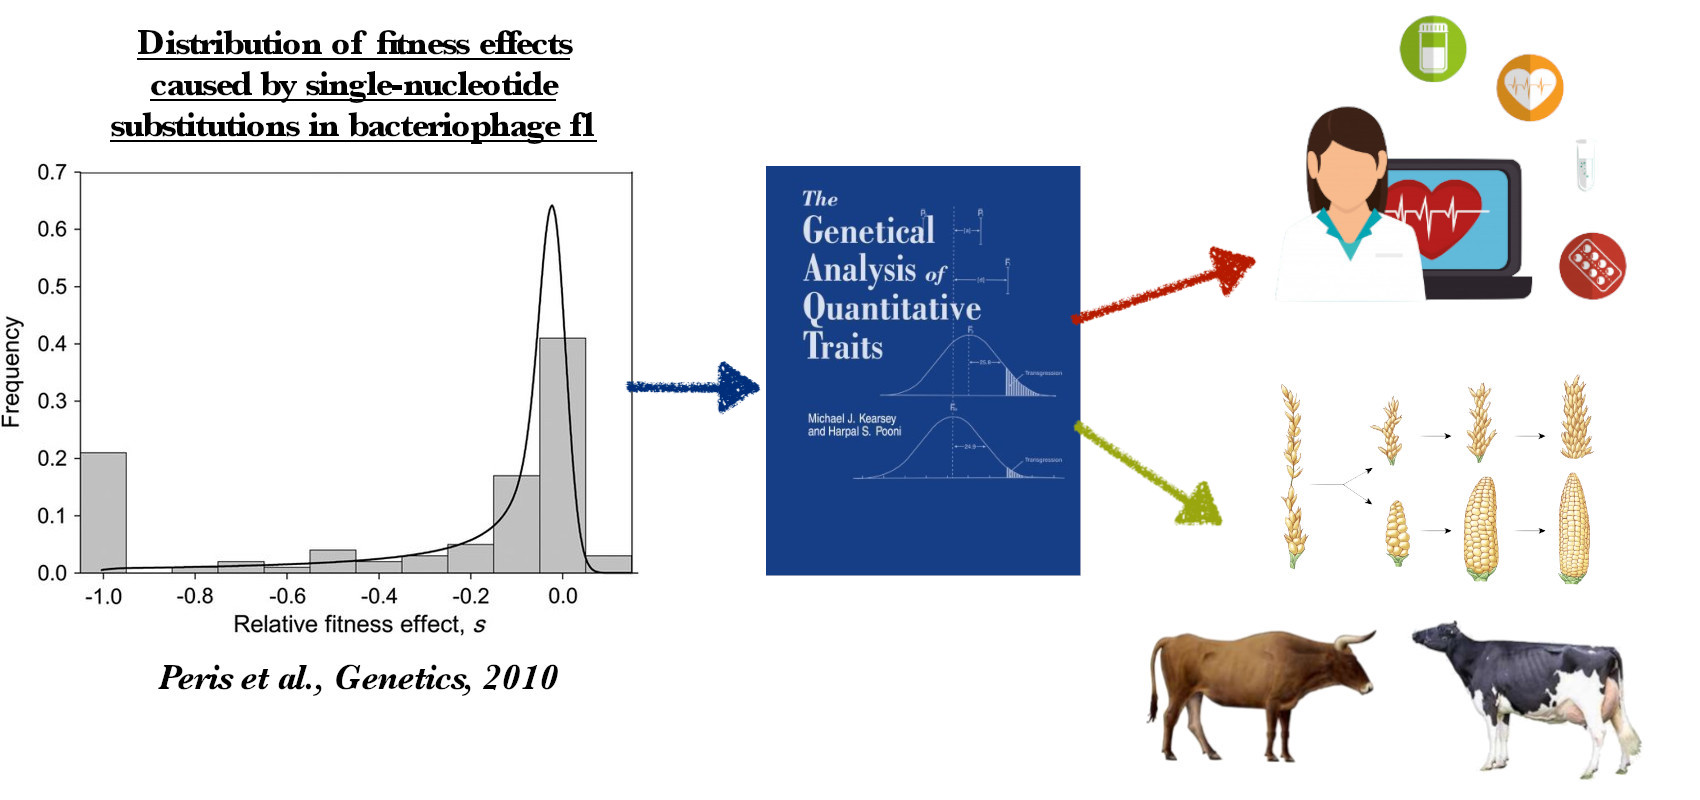
\includegraphics[scale=0.25]{../Img/DFE_phage_2010.jpg}
\end{center} 
  \caption{L'étude de la DFE permet permet l'analyse génétique des traits quantitatifs. Cela a des applications en médecine et en sélection artificielle.}
\end{figure}

Le point de départ de ce projet est un article de Lydia Robert \textit{et al.} \cite{rob} dont l'objectif est précisément d'aider à comprendre l’impact des mutations sur la fitness. En particulier, les auteur.ice.s ont mis au point un protocole permettant pour la première fois de suivre en temps réel les dynamiques d’apparition des mutations et de croissance-fragmentation chez \textit{Escherichia coli}. Dans les expériences classiques d’accumulation de mutations dans des colonies bactériennes, les observations sont moyennées sur plusieurs générations, induisant des biais par l’effet de la sélection naturelle éliminant les mutations trop délétères, voire létales, et par le nombre limité de lignées pouvant être suivies. 

\subsection{Expériences}

Dans l'article de Lydia Robert \textit{et al.} \cite{rob} sont présentés deux types d'expérience dépassant une partie de ces limitations, en se basant sur l'observation de bactéries piégées dans 1000 micro-canaux d'une puce micro-fluidique :
\begin{enumerate}
\item \textbf{microfluidic Mutation Accumulation ($\mu$MA) experiment} : suivi du taux de croissance des bactéries sur de nombreuses générations en supprimant les effets de la sélection naturelle. Le taux de croissance des bactéries représentera la fitness des cellules;
\item \textbf{Mutation Visualization (MV) experiment} : détection en temps réel des mutation apparaissant dans l'ADN bactérien.
\end{enumerate}

\paragraph{Détails de l'expérience $\mu$MA}

Dans cette expérience, les bactéries sont placées dans une \emph{Mother Machine} dans laquelle environ $1500$ cellules-mères se multiplient dans des micro-canaux individuels, leurs descendantes étant évacuées au fur et à mesure. En observant ces cellules au cours du temps, comme représenté dans la figure \ref{fig:microMA} tirée de l'article, on peut reconstruire l'évolution des taux de croissance sur plusieurs générations et essayer d'extraire la part de ces variations due à l'apparition de mutations.

\begin{figure}[h]
  \begin{center}
    \vspace{3mm}
    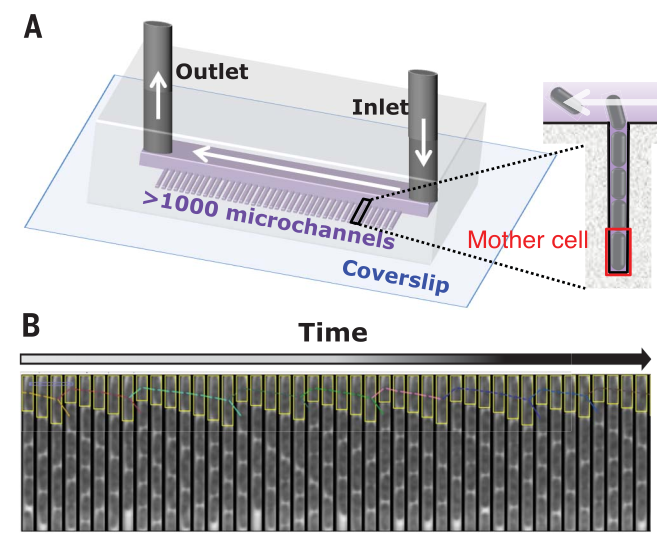
\includegraphics[scale=0.4]{../Img/Schema_microMA.png}
  \end{center} 
  \caption{\label{fig:microMA}$(A)$ Vue d'ensemble de la \emph{Mother Machine} utilisée pour les expériences MV et $\mu$MA. $(B)$ Évolution temporelle de l'état d'un unique canal. La cellule mère, qui est celle dont on mesure le taux de croissance dans l'expérience $\mu$MA, est colorée en jaune.}
\end{figure}

Le dispositif élimine totalement la sélection naturelle, puisque même les cellules-mères mortes suite à des mutations létales sont conservées.

\paragraph{Détails de l'expérience MV}

Dans cette expérience, on se place toujours dans la \emph{Mother Machine} et on observe par fluorescence (figure \ref{fig:MV}) l'apparition de mésappariements entre paires de nucléotides dues à des erreurs de réplication de l'ADN (via l'insertion d'un rapporteur YFP-MutL). En prenant des mutants (\emph{MutH}, \emph{MutT}) dont le système de réparation est dysfonctionnel, on s'assure que toute erreur d'appariement donne à terme une mutation. Les apparitions de taches fluorescentes correspondent donc bien à l'apparition d'une mutation.

\begin{figure}[h]
  \begin{center}
    \vspace{3mm}
    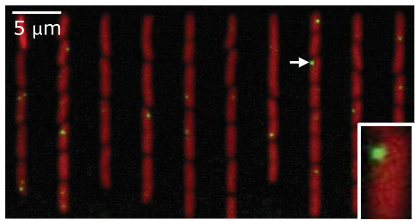
\includegraphics[scale=0.5]{../Img/Schema_MV.png}
  \end{center}
  \caption{\label{fig:MV}Prise de vue reconstituée de l'expérience MV. Les mutations détectées correspondent aux points fluorescents jaunes.}
\end{figure}

À partir de ces expériences, plusieurs questions sont posées dans l'article : est-ce que les mutations sont ponctuelles (dynamique d'apparition poissonnienne) ou arrivent groupées ? Est-ce que les baisses soudaines du taux de croissance sont dues à l’arrivée de mutations délétères isolées ou bien à une accumulation de mutations en interaction ? Quelle est la dynamique d’apparition de mutations létales ? Et, surtout, pour le problème qui nous intéresse: peut-on inférer la DFE ?

\subsection{Modélisation mathématique}

\paragraph{Notations}
On se place dans le cadre de l'expérience $\mu$MA d'accumulation de mutations. On note $W_t$ le taux de croissance au temps $t\geqslant 0$ d'une lignée de cellule, et $N_t$ le nombre de mutations qu'il y a eu sur cette lignée depuis le début de l'expérience. On note \[S_i=\frac{W_{t_{i-1}}-W_{t_i}}{W_{t_{i-1}}}\in\iof{-\infty,1}\] l'effet relatif de la $i^e$ mutation. On a en particulier: 
\begin{equation}\label{mod}
  \frac{W_t}{W_0}=\prod_{i=1}^{N_t}(1-S_i)
\end{equation}
Enfin, on note $\lambda$ le taux de mutation, que l'on suppose constant.

\paragraph{Objectif} Le but du projet est de répondre au problème suivant:
\vspace{5mm}

\boxed{
  \begin{minipage}{0.9\linewidth}
    \textbf{Énoncé du problème:} Estimer la loi des $S_i$ sachant que l'on peut mesurer expérimentalement $W_t$, sachant que $N_t$ suit une loi de Poisson de paramètre $\lambda t$ et sachant que l'on a l'expression \eqref{mod}. Trouver une mesure pertinente pour exprimer l'erreur entre la loi estimée et la loi <<~réelle~>>.
\end{minipage}}


\paragraph{Hypothèses}
On fait les hypothèses suivantes sur les cellules:
\begin{enumerate}
\item Les effets des mutations $S_i$ sont indépendants et identiquement distribués;
\item Les mutations arrivent selon une dynamique poissonnienne;
\item Le taux de mutation $\lambda$ est constant. En particulier, il ne dépend pas du taux de croissance;
\item Le taux de croissance change instantanément après la mutation (on ne prend pas en compte la division des cellules);
\item Les taux de croissance des cellules ne changent que à cause des mutations.
\end{enumerate}

\req{L'hypothèse 1 permet de dire que la DFE, que l'on recherche, est bien définie. Dans la section \ref{ss:dyn_pois}, on montre que l'hypothèse 2 est justifiée expérimentalement.}

\subsection{Dynamique poissonnienne des mutations\label{ss:dyn_pois}}

Afin de tester expérimentalement l'hypothèse d'apparition poissonnienne des mutations, les auteur.ice.s ont évalué les intervalles de temps $\delta$ entre deux apparitions de mutations dans l'expérience de MV. Ces intervalles définissent un processus de Poisson si leurs longueurs suivent une distribution exponentielle et sont indépendantes deux à deux (et en particulier d'un interval $\delta_n$ au suivant $\delta_{n+1}$). La figure \ref{fig:iatime} montre que ces deux critères sont vérifiés, en corrigeant la distribution attendue pour des observations discontinues toutes les 4 minutes. Nous avons répliqué ces résultats dans le notebook \emph{I4\_Replication\_Dynamique-apparition-mutations}\footnote{\url{https://github.com/Jeremy-Andreoletti/MSV_Project_DFE/blob/master/I4_Replication_Dynamique-apparition-mutations}}.

\begin{figure}[h]
  \begin{center}
    \vspace{3mm}
    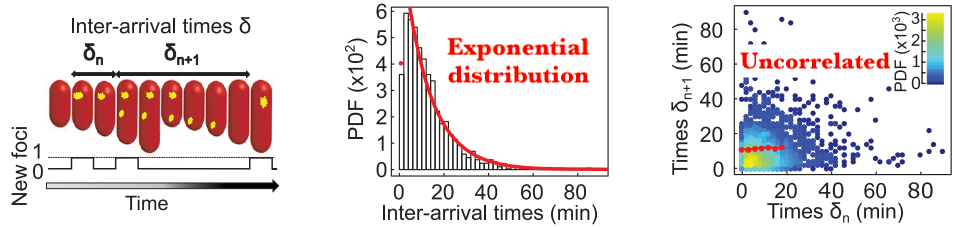
\includegraphics[scale=0.45]{../Img/Interarrival_times.png}
  \end{center}  
  \caption{\label{fig:iatime}Schémas tirés de \cite{rob} montrant que les mutations apparaissent selon un processus de Poisson.}
\end{figure}
\FloatBarrier

De même, on peut vérifier avec la seconde expérience ($\mu$MA) que les mutations létales suivent une dynamique semblable. Cela n'est pas évident a priori, si l'on imagine que certaines mutations ont plus de chances d'être létales quand la cellule a déjà accumulé précédemment des mutation délétères dans des voies partiellement redondantes qui ne peuvent donc plus compenser une nouvelle perte de fonction. Empiriquement, on observe que les courbes de survie (figure \ref{fig:survival}) suivent une courbe exponentielle. On remarque aussi qu'un phénomène de sénescence des cellules commence à émerger, bien visible à partir d'environ 40 heures chez la souche sauvage \emph{WT} qui a peu de mutations. Le phénomène de sénescence peut être corrigé en divisant par le taux de croissance des cellules WT (de taux d'apparition de mutations létales très faible). Après ces corrections, seule la souche MF1 semble s'écarter légèrement d'une trajectoire exponentielle.

\begin{figure}[h]
  \begin{center}
    \vspace{3mm}
    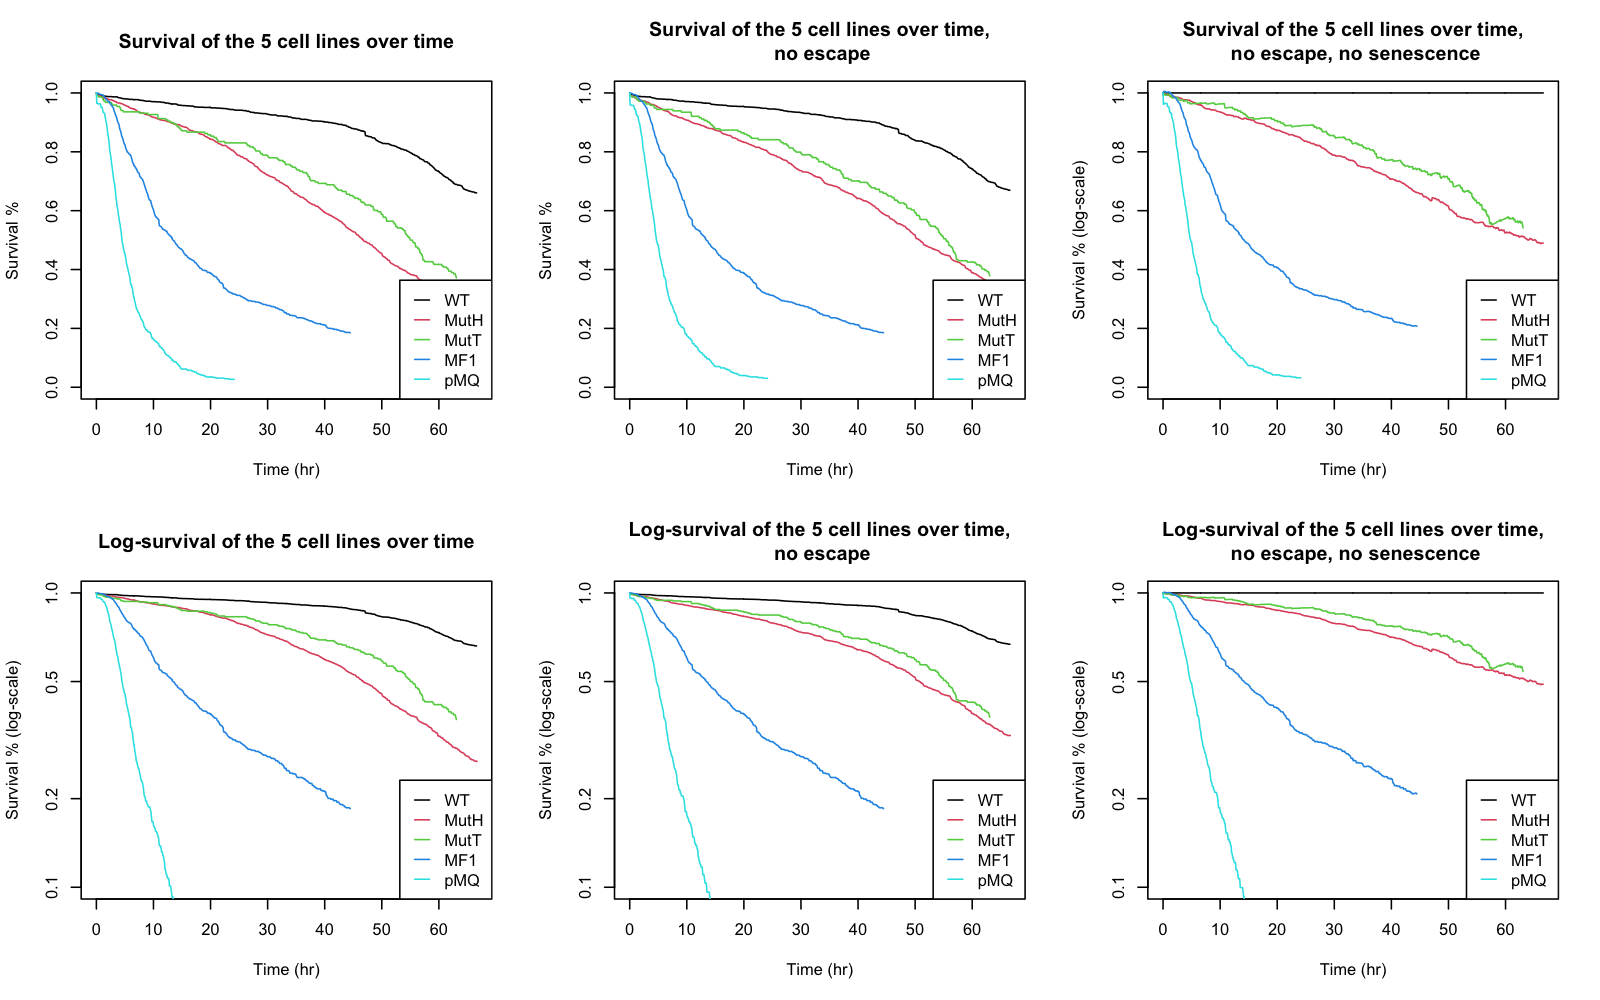
\includegraphics[scale=0.3]{../Img/Survival.png}
  \end{center} 
  \caption{\label{fig:survival}Schéma tiré de notre réplication des résultats, montrant les corrections effectuées pour obtenir une décroissance exponentielle du nombre de cellules au cours du temps. Gauche: sans correction; milieu: suppression des canaux dont les cellules se sont échappées; droite: compensation des cellules qui meurent de vieillesse.}
\end{figure}

\FloatBarrier
\subsection{Tentative naïve pour déterminer la DFE}

Nous avons essayé d'observer directement les variations des taux de croissance dues aux effets combinés des mutations et de la stochasticité des mesures, et si possible corriger cette dernière afin d'obtenir une estimation directe de la DFE. Toutes ces tentatives sont présentées dans le notebook \emph{I5\_DFE-directe\_Sauts-taux-de-croissance}\footnote{\url{https://github.com/Jeremy-Andreoletti/MSV_Project_DFE/blob/master/I5_DFE-directe_Sauts-taux-de-croissance.ipynb}}.

Nous nous basons sur le modèle de bruit multiplicatif dont la pertinence est justifiée dans l'article.
Notons $W_\varepsilon$ le taux de croissance mesuré et $W$ le taux de croissance réel au temps $t$. On suppose que $W_\varepsilon=W(1+\varepsilon)$ où les $\varepsilon_i$, $i\in\En$ sont des variables aléatoires indépendantes, identiquement distribuées, et indépendantes des $W$. On peut alors exprimer les effets relatifs bruités sur la fitness $S_\varepsilon$, avec $W_\varepsilon'$ la mesure de fitness au temps $t'$ suivant :

\[S_\varepsilon=\frac{W_\varepsilon - W_\varepsilon'}{W_\varepsilon} 
= \frac{W(1+\varepsilon) - W'(1+\varepsilon')}{W(1+\varepsilon)}
= 1 - \frac{W'}{W}\frac{1+\varepsilon'}{1+\varepsilon}\]
et donc, comme $\abs{\varepsilon'}$ est très petit:
\[1 - S_\varepsilon \simeq \frac{W'}{W}(1+\varepsilon')(1-\varepsilon)\simeq \frac{W'}{W}(1+\varepsilon'-\varepsilon)\]
Ce calcul montre que le bruit sur l'effet relatif sur la fitness calculé directement est deux fois plus élevé que le bruit sur la mesure. Cela est une première contre-indication à l'efficacité du calcul direct des effets des taux de croissance.

Nous avons tout de même essayé de regarder les distributions de variations relatives des taux de croissance pour les différentes souches de bactéries (figure \ref{fig:VarRel}). Ces distributions de variations relatives de taux de croissance ne sont pas non plus normales, ni même symétrique si on superpose les 2 moitiés (verte et rouge).

\begin{figure}[!h]
  \begin{center}
    \vspace{3mm}
    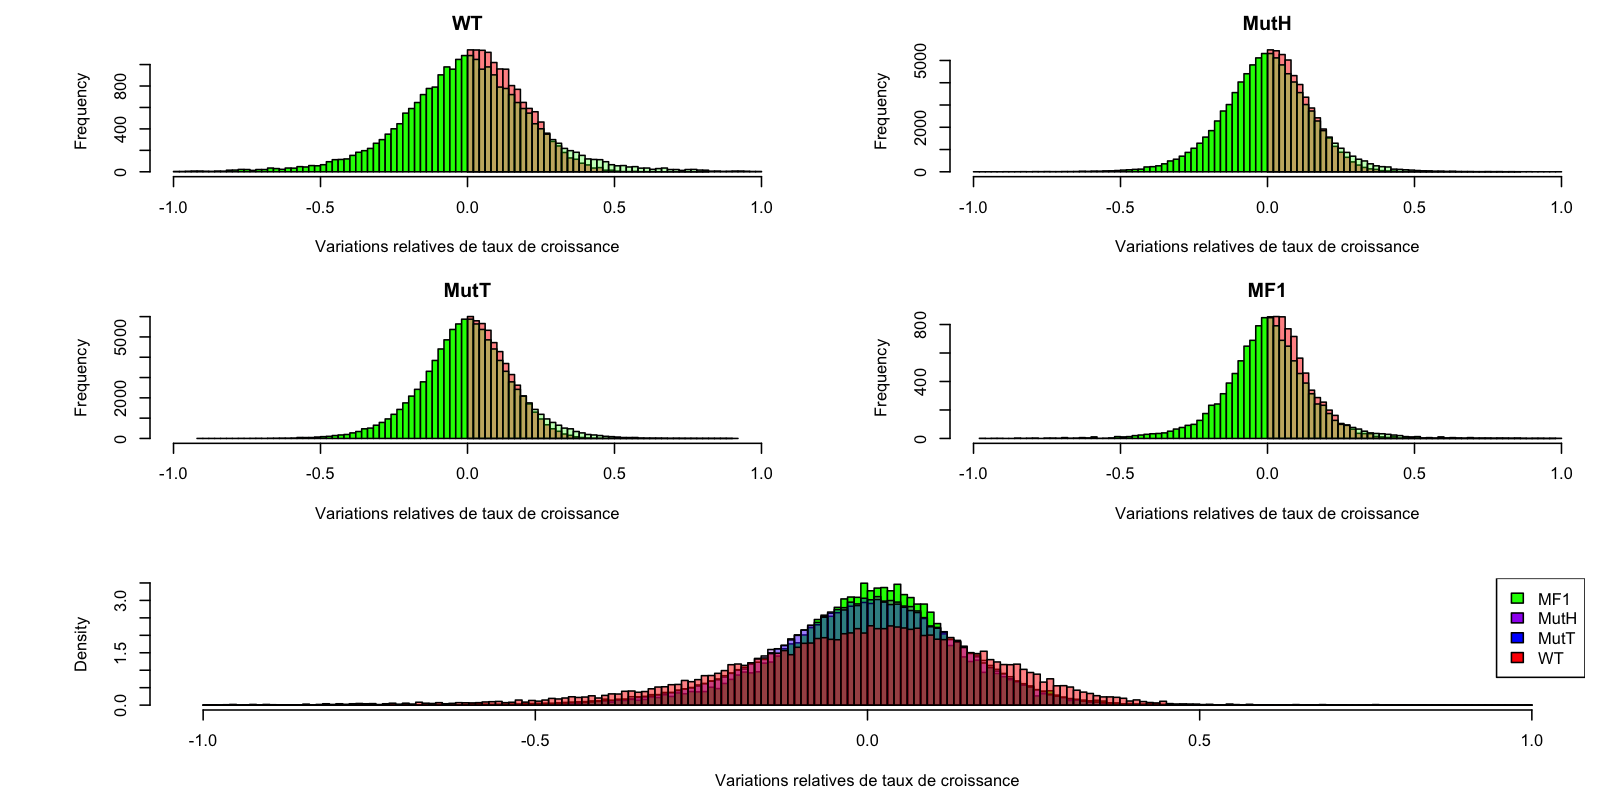
\includegraphics[scale=0.3]{../Img/Variations_relatives_GR.png}
  \end{center} 
  \caption{\label{fig:VarRel}Distribution des variations relatives des taux de croissance observées au cours de l'expérience, pour les différentes souches. Dans chaque cas la partie gauche de la distribution, en verte, a été reflétée de manière à illustrer l'asymétrie de ces distributions.}
\end{figure}

Plus le taux de mutation est faible ($\mu_{WT} < \mu_{MutH} \simeq \mu_{MutT} < \mu_{WT}$) plus la distribution des sauts relatifs de croissance est étalée. La part du bruit devient plus importante que celle du signal.

Malheureusement, les diverses tentatives subséquentes de retirer la distribution WT (quasiment uniquement du bruit) aux autres distributions, ou de faire des régressions pour des taux de mutations croissants se sont avérées être des échecs. Cela confirme la nécessité de faire appel à des outils mathématiques plus poussés afin de reconstruire la DFE.

\FloatBarrier
\section{Simulations}

Nous avons voulu réaliser des simulations aussi proches que possible de l'expérience réelle, en prenant en compte à la fois les mutations impactant les taux de croissance selon une DFE, la croissance des bactéries et le bruit des mesures. Les fonctions et animations associées sont présentées dans le notebook \emph{II\_Simulations}\footnote{\url{https://github.com/Jeremy-Andreoletti/MSV_Project_DFE/blob/master/II_Simulations.ipynb}}.

\begin{figure}[!h]
  \begin{center}
    \vspace{3mm}
    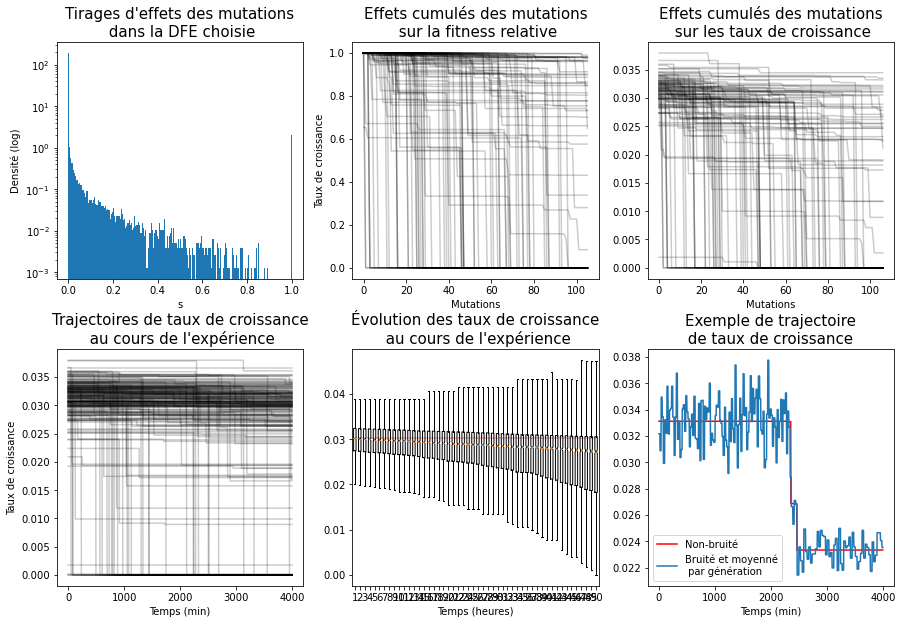
\includegraphics[scale=0.5]{../Img/Simulations.png}
  \end{center} 
  \caption{\label{fig:simulations}Quelques étapes d'une simulation réaliste d'une expérience de croissance bactérienne, dont le taux de croissance est affecté par des mutations selon une DFE donnée et mesuré de manière bruitée}
\end{figure}

Afin d'être les plus réalistes possibles, nos simulations suivent les étapes suivantes (voir figure \ref{fig:simulations}) :
\begin{itemize}
\item Les taux de croissance sont initialisés avec ceux mesurés dans l'expérience (médiane des 10 premières valeurs);
\item Une DFE est tirée dans un mélange de distributions au choix. Ici, nous avons pris la distribution Beta inférée dans l'article (de paramètres $\alpha=0.0074$ et $\beta=2.4$) à laquelle on a rajouté un Dirac en 1 (permettant d'incorporer $1\%$ de mutations létales);
\item Les effets $s$ des mutations sur la fitness sont tirés dans cette DFE pour chacun des 1476 canaux de l'expérience et grand nombre de mutations;
\item L'évolution du taux de croissance, mutation par mutation, est déduite des effets relatifs cumulés des mutations modifiant les taux de croissance initiaux;
\item Les durées entre 2 mutations sont tirées dans une loi exponentielle dont le paramètre est le taux de mutation ($\sim0.32$/heure en se basant sur le mutant \emph{mutH}). Le taux de mutation peut être soit constant dans le temps et entre les cellules, soit être décroissant avec le taux de croissance (le cycle cellulaire et la réplication étant ralentis);
\item À partir des temps d'apparition de chaque mutation on peut ne conserver que celles qui arrivent avant la fin de l'expérience (4000 minutes) et calculer l'évolution du taux de croissance, cette fois au cours du temps;
\item Enfin, le résultat est renvoyé en rajoutant (ou non) un bruit Gaussien multiplicatif à chaque mesure. Ce bruit est ensuite moyenné sur chaque génération de bactérie (comme indiqué dans l'article), en supposant que les bactéries se divisent dès qu'elles ont doublé de taille (bien qu'un modèle de division incrémental serait plus réaliste).
\end{itemize}

\begin{figure}[!h]
  \begin{center}
    \vspace{3mm}
    \includemedia[width=\linewidth, height=0.34\linewidth, 
    activate=pageopen,  passcontext,  transparent,  keepaspectratio,
    addresource=../Video/GrowthRates_noisySimulations_VS_observations.mp4,  flashvars={source=../Video/GrowthRates_noisySimulations_VS_observations.mp4
                  &autoPlay=true
                  &loop=true}]{}{VPlayer.swf}
    \includemedia[width=\linewidth, height=0.34\linewidth, 
    activate=pageopen,  passcontext,  transparent,  keepaspectratio,
    addresource=../Video/GrowthRates_noisySimulationsInterval_VS_observations.mp4,  flashvars={source=../Video/GrowthRates_noisySimulationsInterval_VS_observations.mp4
                  &autoPlay=true
                  &loop=true}]{}{VPlayer.swf}
  \end{center} 
  \caption{\label{fig:animations}Animations montrant l'évolution de la distribution des taux de croissance au cours du temps dans les simulations et l'expérience réelle. La seconde animation affiche un intervalle des valeurs simulées sur 100 réplications.}
\end{figure}

Les animations présentées dans la figure \ref{fig:animations} représentent l'évolution au cours du temps de la distribution des taux de croissance, en comparant les simulations aux données empirique. On observe que l'évolution de la distribution simulée est au début en bonne adéquation avec celle observée. Toutefois, après 40 heures les deux commencent à diverger, probablement à cause du début de la sénescence des cellules, et de la DFE non adaptée (pas de mutations avantageuses, trop peu de mutations fortement délétères).

\FloatBarrier
\section{Problème des moments}

\subsection{Détermination des moments}\label{ss:det_mom}

Dans cette section, nous allons présenter la méthode donnée dans l'article afin d'estimer les moments de la DFE à partir des moments de la loi des $W_t$, $t\geqslant 0$.

Définissons \[E_n(t)=\sum_{k=1}^n(-1)^k\binom{n}{k}\ln\pth{\Esp{W_t^k}}\]

\prop{Pour $t\geqslant 0$ et $n\in\En$: \[E_n(t)=\pth{\lambda\Esp{S^n}}t\]}

\req{En traçant les fonctions $t\mapsto E_n(t)$ (que l'on est capable de calculer à partir des observations de l'expérience $\mu$MA), on devrait obtenir des droites dont les pentes seront directement reliées aux moments de la DFE par un facteur $\lambda$. Dans l'annexe \ref{ann:resultats} et le notebook \emph{III1\_Replication\_Estimation-moments}\footnote{\url{https://github.com/Jeremy-Andreoletti/MSV_Project_DFE/blob/master/III1_Replication_Estimation-moments.ipynb}}, nous montrons que \cite{rob} a bien obtenu des droites et nous expliquons les traitements permettant de reproduire ces résultats, et ainsi estimer les moments de la DFE.}

\begin{proof}
  Tout d'abord, remarquons que, $N_t$ suivant une loi de Poisson de taux $\lambda t$ :
  \begin{align*}
    \Esp{W_t^k}&=\Esp{\Esp{\prod_{i=1}^{N_t}(1-S_i)^k\kt N_t}}\\
    &=\Esp{\Esp{(1-S)^k}^{N_t}}\\
    &=e^{-\lambda t}\sum_{i=0}^{+\infty}\frac{\Esp{(1-S)^k}^i(\lambda t)^i}{i!}\\
    &=e^{-\lambda t}e^{\lambda t\Esp{(1-S)^k}}
  \end{align*}
  Maintenant, nous pouvons calculer:
  \begin{align*}
    E_n(t)&=\sum_{k=1}^n(-1)^k\binom{n}{k}\pth{-\lambda t+\lambda t\Esp{(1-S)^k}}\\
    &=\lambda t\sum_{k=1}^n(-1)^k\binom{n}{k}\pth{\Esp{\sum_{l=0}^k\binom{k}{l}\pth{-S}^l}-1}\\
    &=\lambda t\sum_{k=1}^n\pth{(-1)^k\binom{n}{k}\sum_{l=1}^k(-1)^l\binom{k}{l}\Esp{S^l}}\\
    &=\lambda t\sum_{l=1}^n\Esp{S^l}\pth{\sum_{k=l}^n(-1)^{k+l}\binom{n}{k}\binom{k}{l}}\\
    &=\lambda t\sum_{l=1}^n\Esp{S^l}\pth{\binom{n}{l}\sum_{k=l}^n(-1)^{k+l}\binom{n-l}{k-l}}\\
    &=\lambda t\sum_{l=1}^n\Esp{S^l}\pth{\binom{n}{l}(1-1)^{n-l}}\\
    &=\lambda t\Esp{S^n}
  \end{align*}
\end{proof}




\subsection{Estimation de la DFE}

Nous avons vu dans \ref{ss:det_mom} qu'il était possible de déterminer les moments de la loi de $S$ à partir de la donnée de la distribution des $W_t\vg t\geqslant 0$. Maintenant, nous allons tenter de trouver la loi de $S$ à partir des moments de $S$: cela s'appelle le problème des moments.

\paragraph{Estimation de la fonction caractéristique}

À partir de tous les moments de $S$, on peut calculer la fonction caractéristique $\varphi$ de la loi de $S$, grâce à l'expression suivante:
\[\varphi_S(\xi):=\Esp{e^{i\xi S}}=\Esp{\sum_{k=0}^{+\infty}\frac{(iS\xi)^k}{k!}}=\sum_{k=0}^{+\infty}\frac{(i\xi)^k}{k!}\Esp{S^k}\]
Il est légal d'inverser la somme et l'espérance si l'on fait l'hypothèse que $\abs{S}$ est bornée. En particulier, cette hypothèse est vérifiée si toutes les mutations sont délétères: dans ce cas, $0\leqslant S\leqslant 1$.

On a alors, pour tout $N\in\En$:

\begin{align*}
\varphi_S(\xi):=\Esp{e^{i\xi S}}
&=\sum_{k=0}^{N}\frac{(i\xi)^k}{k!}\Esp{S^k}+\sum_{k=N+1}^{+\infty}\frac{(i\xi)^k}{k!}\Esp{S^k}\\
&= \sum_{k=0}^{N}\frac{(i\xi)^k}{k!}m_k + \sum_{k=0}^{N}\frac{(i\xi)^k}{k!}\pth{\Esp{S^k}-m_k}+\sum_{k=N+1}^{+\infty}\frac{(i\xi)^k}{k!}\Esp{X^k}
\end{align*}
où $m_0,\hdots, m_N$ sont les moments que l'on a estimés par la méthode de la section précédente.

Notons \[\hat{\varphi}_X(\xi)=\sum_{k=0}^{N}\frac{(i\xi)^k}{k!}m_k\] qui est la meilleure estimation que l'on peut avoir de la fonction caractéristique à partir des $N$ premiers moments.

\paragraph{Conventions utilisées pour la transformée de Fourier}

Nous définissons la transformée de Fourier $\fr:L^2(\Er)\to L^2(\Er)$ et la tranformée de Fourier inverse $\fr^{-1}:L^2(\Er)\to L^2(\Er)$ par densité, à partir des expressions:
\[\fr f(\xi)=\int_{\Er}f(x)e^{-ix\xi}\de x\et \fr f(\xi)=\frac{1}{2\pi}\int_{\Er}f(x)e^{ix\xi}\de x\]
définies pour $f\in L^1(\Er)$. On a notamment: \[\fr\circ\fr^{-1}=Id_{L^2(\Er)}\]

\paragraph{Estimation de la DFE}

On remarque que, si la loi de $S$ a une densité $f$:
\[\varphi_X(\xi)=2\pi \mathcal{F}^{-1}f(\xi)\]

À partir de la fonction caractéristique $\varphi_S$, on peut donc trouver la densité $f$ de $S$ :

\[f(x) = \frac1{2\pi} \int_{\mathbb R}\varphi_S(\xi)e^{-ix\xi}\de\xi\]

Seulement, on ne connaît que les $N+1>0$ premiers moments, chacun avec une certaine erreur $(\varepsilon_k)_{0\leqslant k\leqslant N}$. Ainsi, on ne va calculer $\varphi_S(\xi)$ avec une erreur raisonnable que pour $\xi\leqslant A$, ce qui induira une erreur sur l'estimation de $f$.

Notons $\hat{f}$ la fonction que l'on calcule par cette méthode, qui est une estimation de $f$ : 
\begin{equation}\label{dfe1}
  \hat{f}(x) = \frac1{2\pi} \int_{\abs{\xi}\leqslant A}\hat\varphi_S(\xi)e^{-ix\xi}\de\xi
\end{equation}

\subsection{Bornes sur l'erreur commise}

On remarque que l'estimation \eqref{dfe1} de la DFE $f$ contient trois approximations:
\begin{enumerate}
\item l'erreur de régularisation qui consiste à ne pas considérer $\xi>A$;
\item l'erreur sur le calcul de $\hat{\varphi}_S$ qui consiste à ne considérer que les $N$ premiers moments;
\item l'erreur sur l'estimation des moments considérés.
\end{enumerate}
Nous retrouverons ces trois erreurs dans la borne suivante sur l'erreur entre  $\hat{f}$ et $f$:

\prop{Soient $A>0$, $N\geqslant 1$, $k\geqslant 2$. On a alors: \[\qt{\forall x\in\Er} \abs{\hat{f}(x)-f(x)}\leqslant \alpha_1+\alpha_2+\alpha_3\] avec:
\begin{align*}
\alpha_1&=\frac{\dabs{2f^{(k)}}_1}{(k-1)A^{k-1}}\\
\alpha_2&=\frac{A^{N+1}}{\pi(N+1)!}\Esp{S^N(e^{AS-1})}\\
\alpha_3&=\frac{\dabs{\varepsilon(N)}_{\infty}(e^A-1)}{\pi}
\end{align*}
où $\dabs{\varepsilon(N)}_{\infty}$ est l'erreur maximale commise sur le calcul des $N$ premiers moments. }

\begin{proof}
On peut décomposer $f(x)$ selon la régularisation des coefficients $\xi$ et l'estimation de $\varphi_S(\xi)$:

\begin{align*}
f(x) &= \frac1{2\pi} \int_{\mathbb R}\varphi_S(\xi)e^{-ix\xi}\de\xi
= \frac1{2\pi} \int_{\abs{\xi}\leqslant A}\varphi_S(\xi)e^{-ix\xi}\de\xi + \underbrace{\frac1{2\pi} \int_{\abs{\xi} > A}\varphi_S(\xi)e^{-ix\xi}\de\xi}_{a_1}\\
&= \frac1{2\pi} \int_{\abs{\xi}\leqslant A}\pth{\hat{\varphi}_S(\xi)+\sum_{k=0}^{N}\frac{(i\xi)^k}{k!}\pth{\Esp{S^k}-m_k}+\sum_{k=N+1}^{+\infty}\frac{(i\xi)^k}{k!}\Esp{S^k}}e^{-ix\xi}\de\xi + a_1\\
&= \underbrace{\frac1{2\pi} \int_{\abs{\xi}\leqslant A}\hat{\varphi}_S(\xi)e^{-ix\xi}\de\xi}_{\hat f(x)}
+ a_1
+ \underbrace{\frac1{2\pi}\int_{\abs{\xi}\leqslant A}\sum_{k=N+1}^{+\infty}\frac{(i\xi)^k}{k!}\Esp{S^k}e^{-ix\xi}\de\xi}_{a_2}\\
&\esp+ \underbrace{\frac1{2\pi}\int_{\abs{\xi}\leqslant A}\sum_{k=0}^{N}\frac{(i\xi)^k}{k!}\pth{\Esp{S^k}-m_k}e^{-ix\xi}\de\xi}_{a_3}\\
&= \hat{f}(x) + a_1 + a_2 + a_3
\end{align*}

On obtient donc comme majoration de l'erreur d'approximation de $f$, pour $x\in\Er$:
\[\abs{f(x)-\hat{f}(x)} = \abs{a_1 + a_2 + a_3}\leqslant |a_1| + |a_2| + |a_3|\]
où

\begin{itemize}
\item $\abs{a_1}$ est l'erreur que l'on commet en omettant de calculer $\varphi_S(\xi)$ pour $\xi>A$ (erreur de régularisation). %On a:
  %\begin{align*}
  %2\pi\alpha_1&\leqslant \int_{\abs{\xi}>A}\abs{\varphi_S(\xi)e^{-ix\xi}}\de\xi=\int_{\abs{\xi}>A}\abs{\varphi_S(\xi)}\de\xi
  %\end{align*}

\[\abs{a_1} = \frac1{2\pi} \abs{\int_{\abs{\xi} > A}\varphi_S(\xi)e^{-ix\xi}\de\xi}\]

  Pour tout $k\geqslant 2$: $2\pi\pth{\mathcal{F}^{-1}(f^{(k)})}(\xi)=(i\xi)^k\varphi(\xi)$ donc:
  \begin{align*}
    \abs{a_1}&=\abs{\int_{\abs{\xi}>A}\frac{1}{(i\xi)^k}\mathcal{F}^{-1}(f^{(k)})(\xi)e^{-ix\xi}\de\xi}\\
    &\leqslant \int_{\abs{\xi}>A}\frac{1}{\abs{\xi}^k}\underbrace{\abs{\mathcal{F}^{-1}(f^{(k)})(\xi)}}_{\leqslant\dabs{f^{(k)}}_{1}}\de\xi\\
    &\leqslant 2\dabs{f^{(k)}}_{1}\int_{\xi>A}1/(\xi^k)\de\xi
  \end{align*}

  On a donc, pour tout $k\geqslant 2$:
  \[\abs{a_1}\leqslant \alpha_1=\frac{2\dabs{f^{(k)}}_{1}}{(k-1)A^{k-1}}\] %Pour que cette borne soit bonne, il faut d'une part faire certaines hypothèse sur $f$, d'autre part prendre $A$ assez grand;
\item $\abs{a_2}$ est l'erreur que l'on commet en omettant dans notre calcul les moments d'ordre plus grand que $N+1$:

\[\abs{a_2} = \frac1{2\pi}\abs{\int_{\abs{\xi}\leqslant A}\sum_{k=N+1}^{+\infty}\frac{(i\xi)^k}{k!}\Esp{S^k}e^{-ix\xi}\de\xi}\]

On a :
  \begin{align*}
    2\pi\abs{a_2}&\leqslant \int_{-A}^A\abs{\sum_{k=N+1}^{+\infty}\frac{(i\xi)^k}{k!}\Esp{S^k}}\de\xi\\
    &\leqslant  \int_{-A}^A\sum_{k=N+1}^{+\infty}\frac{\abs{\xi}^k}{k!}\Esp{S^k}\de\xi=2 \int_{0}^A\sum_{k=N+1}^{+\infty}\frac{\xi^k}{k!}\Esp{S^k}\de\xi\\
    &\leqslant 2\sum_{k=N+1}^{+\infty}\frac{A^{k+1}}{(k+1)!}\Esp{S^k}=2\Esp{\frac{1}{S}\sum_{k=N+1}^{+\infty}\frac{(AS)^{k+1}}{(k+1)!}}\\
  \end{align*}
  D'après la formule de Taylor avec reste intégral:
  \begin{align*}
    \sum_{k=N+2}^{+\infty}\frac{(AS)^{k}}{k!}&=e^{AS}-\sum_{k=0}^{N+1}\frac{(AS)^{k}}{k!}\\
    &=\sum_{k=0}^{N+1}\frac{(AS)^{k}}{k!}+\int_{0}^{AS}\frac{(AS-t)^{N+1}e^t}{(N+1)!}\de t-\sum_{k=0}^{N+1}\frac{(AS)^{k}}{k!}\\
    &=\int_{0}^{AS}\frac{(AS-t)^{N+1}e^t}{(N+1)!}\de t = \frac{(AS-t)^{N+1}(e^{AS}-1)}{(N+1)!}
  \end{align*}
  d'où:
  \begin{align*}
    \abs{a_2}\leqslant \alpha_2= 2\Esp{\frac{(AS)^{N+1}(e^{AS}-1)}{2\pi S(N+1)!}}=\frac{A^{N+1}}{\pi(N+1)!}\Esp{S^N(e^{AS}-1)}
  \end{align*}

 % Pour que cette borne soit bonne, il faut prendre $A$ assez petit et $N$ assez grand;
\item $\abs{a_3}$ est l'erreur que l'on commet qui provient des erreurs sur le calcul des moments.

\[\abs{a_3} = \frac1{2\pi}\abs{\int_{\abs{\xi}\leqslant A}\sum_{k=0}^{N}\frac{(i\xi)^k}{k!}\pth{\Esp{S^k}-m_k}e^{-ix\xi}\de\xi}\]

On a:
  \begin{align*} 
    2\pi\abs{a_3}&\leqslant \int_{-A}^A\sum_{k=0}^{N}\abs{\frac{(i\xi)^k}{k!}\pth{\Esp{S^k}-m_k}e^{-i\xi x}}\de\xi\\
    &\leqslant 2\dabs{\varepsilon}_{\infty}\int_{0}^A\sum_{k=0}^{N}\xi^k/(k!)\de\xi\\
    &\leqslant 2\dabs{\varepsilon}_{\infty}\int_{0}^Ae^{\xi}\de\xi
  \end{align*}

  Avec : $$\dabs{\varepsilon}_{\infty} = \max_{k=0,\dots,N} \abs{\Esp{S^k}-m_k}$$

  On a donc:
  \[\abs{a_3}\leqslant \alpha_3= \frac{\dabs{\varepsilon}_{\infty}(e^A-1)}{\pi}\]
\end{itemize}
\end{proof}


\paragraph{Optimisation du paramètre A}

On remarque que $\alpha_1$ diminue quand $A$ augmente, mais $\alpha_3$ augmente quand $A$ augmente. La proposition suivante donne la borne que l'on obtient lorsque l'on prend le meilleur compromis pour $A$ (dans un cas très favorable).

\prop{Supposons que :
\begin{itemize}
\item l'on soit capable de calculer un nombre arbitrairement grand de moments de $f$ avec une erreur bornée par $\varepsilon>0$;
\item il existe $k\in\En$ tel que $d_k=\dabs{f^{(k)}}_1<+\infty$;
\end{itemize}
Alors on a, pour tout $x\in\Er$:
\[\abs{f(x)-\hat{f}(x)}\sim \abs{\frac{1}{\pi\ln(\varepsilon)}}\comment{quand $\varepsilon\to 0$}\]
}

\begin{proof} On traite d'abord le cas particulier $k=2$, pour introduire les idées.
\begin{enumerate}
\item Cas particulier $k=2$: on a donc une erreur que l'on peut majorer par
\[\alpha_1+\alpha_2+\alpha_3 \leqslant \alpha_N(A)=\frac{2d_2}{A}+\frac{A^{N+1}}{(N+1)!\pi}\Esp{S^N(e^{AS}-1)}+\frac{\dabs{\varepsilon}_{\infty}(N)(e^A-1)}{\pi}\]

Supposons que l'on soit capable de prendre $N\to\infty$, avec une erreur sur les moments $\dabs{\varepsilon}_{\infty}(N)$ bornée par $\varepsilon>0$. De cette manière, on a $\alpha_2=0$. Posons $x=2d_2$ et $y=\varepsilon/\pi$. On a alors:
\[\alpha_N(A)\xrightarrow{N\to\infty}\alpha(A)=x/A+y(e^A-1)\]
donc $\alpha'(A)=-x/A^2+ye^A$. On veut $A$ tel que $\alpha$ soit minimum, c'est-à-dire $\alpha'(A)=0$ d'où:
\[A^2e^A=x/y\]
On obtient alors le paramètre $A$ qui minimise la borne : 
\[A = 2W\pth{\frac{\sqrt{x/y}}2} = 2W\pth{\sqrt{\frac{2\pi d_2}{4 \varepsilon}}}\]
avec $W$ la fonction W de Lambert telle que $z=W(z)e^{W(z)}$.

\item Pour $k$ général, avec les mêmes calculs, on trouve que $\alpha'(A)=-\frac{2d_k}{A^k}+ye^A$, ce qui permet de déduire l'expression du meilleur $A$:
\[A=kW\pth{\frac{1}{k}\pth{\frac{2\pi d_k}{\varepsilon}}^{1/k}}\]

\item (FAUX ?) Regardons maintenant le comportement de $A$ quand $\varepsilon\to 0$.
  Comme, quand $z\to\infty$:
  \[W(z)=\ln z-\ln\ln z+o(1)\]
  on a
  \[A_\varepsilon=\ln\pth{\frac{2\pi d_k}{k\varepsilon}}-\ln\ln\pth{\frac{2\pi d_k}{4(k-1)\varepsilon}}+o(1)= \ln(1/\varepsilon)-\ln\ln(1/\varepsilon)+o(1)\] 
%\[A_\varepsilon \mathop{\sim}\limitS_{\varepsilon\to0} \ln\pth{\frac{d_k}{8(k-1)\pi\varepsilon}}\sim \ln(1/\varepsilon)\]
d'où :
\[\alpha(A_\varepsilon)=\frac{\varepsilon}{\pi}(e^{A_\varepsilon}-1) + \frac{x}{{A_\varepsilon}^{k-1}}=\frac{\varepsilon}{\pi}e^{A_{\varepsilon}}+o(1)=\frac{1}{\pi\ln\pth{\frac{1}{\varepsilon}}}+o(1)\]
%\[\alpha(A_\varepsilon)=y(e^{A_\varepsilon}-1) + \frac{x}{{A_\varepsilon}^{k-1}} &\mathop{\sim}\limitS_{\varepsilon\to0} -\frac{d_2k^k}{2\pi^2\ln(\varepsilon)^k}\]
d'où, quand $\varepsilon\to 0$:
\[\alpha(A_\varepsilon)\sim \abs{1/(\pi\ln(\varepsilon))}\]
ce qui permet de conclure la proposition. 
\end{enumerate}
\end{proof}


\paragraph{Commentaires}

Nous pouvons faire les remarques et les commentaires suivants:
\begin{enumerate}
\item On est capable de borner la norme infinie entre la DFE réelle $f$ et la DFE estimée $\hat{f}$. Les bornes que l'on obtient ne sont pas optimales.
\item Sous des hypothèses très favorables, la norme infinie se comporte comme $\abs{\frac{1}{\ln\varepsilon}}$, ce qui est une décroissance très lente de la borne (d'autant plus qu'il est largement exagéré de supposer que l'on sera capable de calculer tous les moments avec une grande précision);
\item Toutefois, la norme infinie n'est pas forcément la plus pertinente dans notre situation. On pourrait penser à d'autres méthode pour mesurer la distance entre ces deux distributions: par exemple, la norme $L^2$, la distance de Kolmogorov, ou la divergence de Kullback-Leibler.
\end{enumerate}

L'objectif de la partie \ref{s:edp} est de présenter une nouvelle méthode pour estimer la DFE.


\FloatBarrier
\section{Étude d'une EDP\label{s:edp}}

Dans cette partie, nous présentons une modélisation du problème par une EDP sur la densité de la loi de $\ln W_t$. À partir de l'EDP, nous pourrons fournir une expression explicite de la loi de $\ln (1-S)$.

Nous commencerons par introduire \eqref{edp}, puis en déduirons une expression explicite pour la loi de $\ln(1-S)$; nous finirons par faire le lien avec un problème de fragmentation.

\subsection{Nouveau point de vue sur le problème}

\paragraph{Transformations initiales}

D'après \eqref{mod}, on a, tant que $W_t>0$: \[\ln W_t=\sum_{i=1}^{N_t}\ln(1-S_i)\]

On fait les deux hypothèses suivantes:
\begin{enumerate}
\item Pour tout $t>0$, la loi de $\ln W_t$ peut s'écrire:
  \[m(t)\delta_{-\infty}+u(t,\cdot)\]
  où $m(t)$ représente la probabilité qu'une cellule soit morte au temps $t$, et où $u(t,\cdot)\in C^{\infty}(\Er)$ est la densité de la loi de $\ln W_t$ en omettant les cellules mortes: ainsi, $\int_{\Er}u(t,\cdot)=1-m(t)$;
\item La loi de $\ln (1-S)$ peut s'écrire:
  \[\mu\delta_{-\infty}+f(\cdot)\]
  où $\mu$ est la proportion de mutations létales et $f(\cdot)
  \in C^{\infty}(\Er)$ est la <<~densité~>> de la loi de $\ln(1-S)$ sans prendre en compte les mutations létales: ainsi, $\int f=1-\mu$.
\end{enumerate}

Remarquons tout de suite que l'on peut déduire la DFE à partir de la donnée de $f$ et de la fraction de mutations létales, mesurée directement dans l'expérience \emph{MA}.

\paragraph{Introduction du modèle}

Soit $\lambda$ le taux de mutation. Considérons:
\[\dr_tu(t,x)=\lambda\pth{\int_{\Er}f(x-y)u(t,y)\de y-\int_{\Er}f(y)u(t,x)\de y}-\lambda\mu u(t,x)\]

Cette expression est plutôt naturelle ; elle peut se comprendre ainsi:
\begin{align*}
&\esp\text{changement de densité de fitness entre $t$ et $t+\de t$}\\
&=\text{taux de mutations}\times\pth{\text{bactéries qui arrivent sur ma fitness}-\text{bactéries qui partent de ma fitness}}\\
&-\text{bactéries qui meurent}
\end{align*} 
où $\lambda\mu$ est le taux de mortalité. 

Faisons quelques transformations pour simplifier l'expression. Comme $\int_{\Er}f(y)\de y = 1-\mu$:

\[\dr_tu(t,x)=\lambda\pth{\int_{\Er}f(x-y)u(t,y)\de y-(1-\mu)u(t,x)}-\lambda\mu u(t,x)\] 
soit:
\[\dr_tu(t,x)=\lambda (f*u(t))(x)-\lambda u(t,x)\] 
que l'on notera, en notant $u_t(\cdot)=(u(t))(\cdot)=u(t,\cdot)$:
\begin{equation}\label{edp}
  \dr_tu_t(x)=\lambda (f*u_t)(x)-\lambda u_t(x)
\end{equation}

\paragraph{Vérification}

On veut vérifier que cette EDP est crédible. Pour cela, on peut par exemple vérifier que le nombre total de cellules $N(t)$ décroît comme $\exp(-\lambda\mu t)$:

\begin{align*}
    N'(t)=\dr_t\pth{\int_{\Er}u(t,x)\de x}&=\int_{\Er}\dr_tu=\lambda \int_{\Er}\pth{\int_{\Er}f(y)(u(t,x-y)-u(t,x))\de y-\mu u(t,x)}\de x\\
    &=\lambda\int_{\Er}f(y)\pth{\int_{\Er}u(t,x-y)\de x-\int_{\Er}u(t,x)\de x}\de y-\lambda\mu\int_{\Er}u(t,x)\de x\\
    &=-\lambda\mu\int_{\Er}u(t,x)\de x=-\lambda\mu t
\end{align*}
ce qui donne, comme prévu, une décroissance malthusienne au taux $\lambda\mu$ (taux de mutation $\times$ proportion de mutations létales) du nombre total de cellules:
\[N(t)=e^{-\lambda\mu t}N(0)\]

\paragraph{Estimation de la DFE}

On peut mesurer $u$ et on aimerait estimer $f$, en sachant que l'EDP ci-dessus est vérifiée: en quelque sorte, on connaît donc la solution mais on ne connaît pas l'EDP. On a la proposition suivante:
\prop{Supposons que $f\in L^2(\Er)$. Soit $u\in C^1(\Er_+\times \Er,\Er)$ une solution classique de \eqref{edp}. Supposons que, pour tout $t\geqslant 0$, $u_t\in \mathcal{S}(\Er)$ et que $\fr u_t$ ne s'annule pas. \\Alors, pour tout $x\in\mathbb{R}$:
  \begin{equation}\label{edp_sol}
    f(x)=\fr^{-1}\pth{\xi\mapsto\frac{\dr_t\pth{\fr u_t(\xi)}}{\lambda\fr u_t(\xi)}+1}    
  \end{equation}
}

\begin{proof}
  En prenant la transformée de Fourier des deux côtés dans \eqref{edp}, on a:
\[\fr \pth{\dr_tu_t}(\xi)=\lambda \fr f(\xi)\fr {u_t}(\xi)-\lambda\fr u_t(x)\]
Comme $u_t\in \mathcal{S}(\Er)$, on a $\dr_t\fr(u_t)=\fr(\dr_tu_t)$, donc:
\[\pth{\dr_t\fr u_t}(\xi)=\lambda \fr f(\xi)\fr {u_t}(\xi)-\lambda\fr u_t(x)\]
et, comme $\fr u_t$ ne s'annule pas:
\begin{align*}
\fr f(\xi)&=\frac{\dr_t\fr u_t(\xi)}{\lambda \fr u_t(\xi)}+1
\end{align*}
Enfin, comme $f\in L^2(\Er)$, on obtient \eqref{edp_sol}.

\end{proof}


%\paragraph{Vérification 2: Comparaison avec la formule de la diapositive}
%
%Avec d'autres calculs, on trouve:
%\[g(x)=\mathcal{F}^{-1}\pth{1+\frac{1}{\lambda t}\Esp{e^{-i\xi Y_t}}}=\mathcal{F}^{-1}\pth{1+\frac{1}{\lambda t}\fr{u_t(\xi)}}=^?\delta_0+\frac{1}{\lambda t}u_t\] où $Y_t=W_t/W_0$ et où $g$ est la densité de $1-S$. Ainsi, en principe, pour $e^y=x>0$,
%\[g(x)=f(\ln x)/x \ou f(y)=e^yg(e^y)\]
%
%On n'a pas encore réussi à montrer que les deux fonctions coïncident (la transformée de Fourier d'une composition nous pose problème).
%


\subsection{Détermination de la DFE à partir de \eqref{edp_sol}\label{ss:det_dfe}}

L'expression \eqref{edp_sol} donne une forme explicite pour $f(x)$. Il faut, pour l'exploiter, être capable de calculer la valeur, pour chaque $\xi$, de
\[a_{\xi}=\frac{\dr_t\fr u_t(\xi)}{\fr u_t(\xi)}\]

Il est intéressant de remarquer que $a_{\xi}\in\Ce$ ne dépend pas du temps. Cela permet d'affirmer que:
\[\fr u_t(\xi)=e^{a_{\xi}t}\fr u_0(\xi)\] et donc:
\[\abs{\fr u_t(\xi)}=e^{\Re(a_{\xi})t}\abs{\fr u_0(\xi)} \et \arg\pth{\fr u_t(\xi)}=\arg{\fr u_0(\xi)}+t\Im(a_{\xi})\]

On a donc deux expressions valables pour tout $t\in \Er_+$:
\begin{align}
  \ln\abs{\fr u_t(\xi)}&=\ln\abs{\fr u_0(\xi)}+t\times\Re(a_{\xi})\label{re_a}\\
  \arg\pth{\fr u_t(\xi)}&=\arg{\fr u_0(\xi)}+t\times\Im(a_{\xi})\label{im_a}
\end{align}

\paragraph{Vérification} Dans l'annexe \ref{ann:verif} et le notebook \emph{IV2\_DFE-EDP-Fourier\_Verifications}\footnote{\url{https://github.com/Jeremy-Andreoletti/MSV_Project_DFE/blob/master/IV2_DFE-EDP-Fourier_Verifications.ipynb}}, nous avons tracé les fonctions de $t$ \eqref{re_a} et \eqref{im_a}, afin de vérifier qu'il s'agit de fonctions affines. Pour $\xi\leqslant 10$, on obtient des fonctions affines dont les pentes donnent respectivement la partie réelle et la partie imaginaire de $a_{\xi}$. Cependant, pour $\xi>20$, on n'obtient plus de droites. Ainsi, pour l'estimation de la DFE, nous n'avons considéré que les valeurs de $\xi$ inférieures à une certaine valeur $\xi_{max}$. Cela revient à tronquer la transformée de Fourier, et donc nous donne une DFE <<~trop régulière~>> . Cette régularisation est de toute manière nécessaire pour éviter tout phénomène de sur-apprentissage.

\paragraph{Estimation de la DFE}

[ATTENDRE D'AVOIR DES RESULTATS COMPLETS POUR PRESENTER ICI DES DFE]

Voir notebook \emph{IV2\_DFE-EDP-Fourier\_Estimation-complete}\footnote{\url{https://github.com/Jeremy-Andreoletti/MSV_Project_DFE/blob/master/IV2_DFE-EDP-Fourier_Estimation-complete.ipynb}}.

\subsection{Lien avec un problème de fragmentation}

\paragraph{Présentation du problème de fragmentation}
Nous présentons ici une transformation de \eqref{edp} qui est étudiée dans \cite{md1}, \cite{md2} dans le cadre d'un problème de fragmentation. Un problème de fragmentation vise à étudier la distribution des tailles de cellules lors de divisions cellulaires successives. L'intérêt du problème réside dans le fait que les cellules ne se divisent pas toujours en leur milieu, mais plutôt en un point aléatoire.

On note $k(x,y)$ la densité de probabilité pour une cellule de longeur $x$ de se diviser en une cellule de longueur $y$ et une cellule de longueur $x-y$. Le noyau de fragmentation $k$ vérifie alors \[k(x,y)=k(x,x-y)\esp \int_0^xk(x,y)\de y=1\]

Un problème intéressant, par exemple, est de savoir si $k$ est bimodal ou non (\ie: si les cellules ont tendance à se diviser en deux cellules de tailles à peu près égales, ou bien si une cellule fille a tendance à être beaucoup plus grosse que l'autre).

Ce modèle est très proche du nôtre: jusqu'à présent, les cellules changeaient de taux de croissance; maintenant, les cellules changent de taille.

La seule véritable différence avec notre modèle est qu'une cellule se divise nécessairement en une cellule plus petite et une cellule plus grande; cependant, cette différence n'est pas fondamentale: en effet, d'après \cite{rob}, il est tout à fait légitime de supposer que l'immense majorité des mutations sont délétères, ce qui revient à négliger les mutations bénéfiques.

\paragraph{Mise en équation} 

Un cas particulier de l'équation étudiée dans \cite{md1}, \cite{md2} est:
\begin{equation}\label{edp_frag}
\dr_tv(t,x)=\int_x^{+\infty}k\pth{\frac{x}{y}}v(t,y)\de y-v(t,x)
\end{equation}


\paragraph{Comparaison avec notre modèle}

Maintenant, nous allons montrer que \eqref{edp_frag} est une version multiplicative de \eqref{edp}.  Considérons $v(t,\cdot)$ la densité de la loi de $W_t$ et $g$ la densité de $1-S$. Posons $x'=e^x$: on a alors $x'v(t,x')=u(t,x)$. Avec le changement de variable $y'=e^y$, on a:
\begin{align*}
  \dr_t(x'v(t,x'))
  &=\lambda\int_{\Er}f(x-y)u(t,y)\de y-\lambda u(t,x)\\
  %&=\lambda\int_{\Er_+}\frac{f(x-\ln y')}{y'}u(t,\ln(y'))\de y'-\lambda u(t,x)\\
  &=\lambda\int_{\Er_+}\frac{1}{y'}f(\ln(x')-\ln(y'))u(t,\ln(y'))\de y'-\lambda u(t,x)\\
  &=\lambda\int_{\Er_+}\frac{y'x'}{y'}g(x'/y')v\pth{t,y'}\de y'-\lambda\pth{x'v(t,x')}
\end{align*}
donc 
\[\dr_tv(t,x')=\lambda\int_{\Er_+}g(y)v\pth{t,\frac{x'}{y}}\de y-\lambda v(t,x')\]
ce qui est équivalent à \eqref{edp_frag}.

\req{Finalement, on trouve que \eqref{edp} est une somme car on a transformé le produit \eqref{mod} en somme en prenant le logarithme.}


\paragraph{Résultat en temps long} L'intérêt de comparer notre problème au problème de fragmentation étudié dans \cite{md1}, \cite{md2} est que ces articles ont obtenu des résultats sur le comportement en temps long des solutions. Dans notre cas précis, il est montré que la distribution des taux de croissance (ou des tailles de cellules) converge vers un Dirac en 0. 

Malheureusement, nous ne pouvons pas exploiter ce résultat en temps long car le temps de l'expérience n'est pas assez <<~long~>> pour que l'on puisse affirmer que l'on observe un comportement asymptotique. Nous avons pu, tout de même, faire tourner notre simulation pendant très longtemps et constater que la distribution convergeait effectivement vers un Dirac en 0.

Dans le cas où le taux de division \emph{dépend de la taille de la cellule} ($\lambda$ est de la forme $x^{\gamma}$, où $x$ est la taille de la cellule et $0<\gamma<1$), \cite{md2} montre que la distribution converge vers une distribution particulière, qui n'est pas forcément un Dirac. Il y a donc une stationnarité qui apparaît. Ce résultat peut être intéressant dans le cas où nous aimerions faire évoluer notre modèle vers un modèle qui prendrait en compte le fait que les cellules qui croissent lentement ont un métabolisme plus lent et, par conséquent, subissent moins de mutations.


%\subsection{Temps court, temps long ?}
% du coup on n'aura sans doute pas le temps de traiter ça en détail.

\section{Conclusion}


\begin{thebibliography}{1}

\bibitem{mac}
  Trudy F. C. Mackay, Eric A. Stone, Julien F. Ayroles,
  \emph{The genetics of quantitative traits: challenges and prospects}, Nature Reviews Genetics, 565–577, 2009
\bibitem{rob}
  Robert et al.,
  \emph{Mutation dynamics and fitness effects followed in single cells}, Science 359, 1283–1286, 16 March 2018
\bibitem{md1}
  Doumic, Escobedo,
  \emph{Time asymptotics for a critical case in fragmentation and growth-fragmentation equations}, submitted 2015
\bibitem{md2}
  Beal et al.,
  \emph{The Division of Amyloid Fibrils: Systematic Comparison of Fibril Fragmentation Stability by Linking Theory with Experiments}, iScience, 25 September 2020
\end{thebibliography}





\newpage

\appendix

\FloatBarrier
\section{Annexe: Présentation des résultats}\label{ann:resultats}

Nous avons répliqué certains résultats dans des notebooks disponibles sur \url{https://github.com/Jeremy-Andreoletti/MSV_Project_DFE}.
%TEST INCLUSION DE PDF
%\includepdf[pages=-]{Notebooks_tex/Replication_Moments_Estimation.pdf}

\paragraph{Commentaires sur les figures} La figure \ref{lines}, tirée de \cite{rob}, présente des graphes de $E_n(t)$. Dans \ref{ss:det_mom}, on a démontré que l'on s'attendait à obtenir des droites de pente $\lambda\Esp{S^n}$: les droites que l'on obtient sont très satisfaisantes. On peut effectuer à partir des ces droites des régressions linéaires pour estimer  les pentes $\lambda\Esp{S^n}$ de ces droites. Les résultats obtenus dans \cite{rob} sont présentés dans le tableau \ref{slopes} pour un nombre plus grand de souches et de moments. Enfin, le tableau \ref{moments} présente des estimations de la moyenne, de l'écart-type, du coefficient d'asymétrie et de la kurtosis pour les DFE de trois souches (\emph{mutH}, \emph{mutT}, \textbf{MF1}). Ces moments particuliers permettent d'obtenir des indices qualitatifs sur la forme des DFE: par exemple, comme le coefficient d'asymétrie et la kurtosis sont très élevés, on s'attend à ce que les DFE soient très piquées et très asymétriques, \ie: très peu de mutations sont très délétères, la plupart des mutations sont quasiment neutres.


\begin{figure}[h]
  \begin{center}
    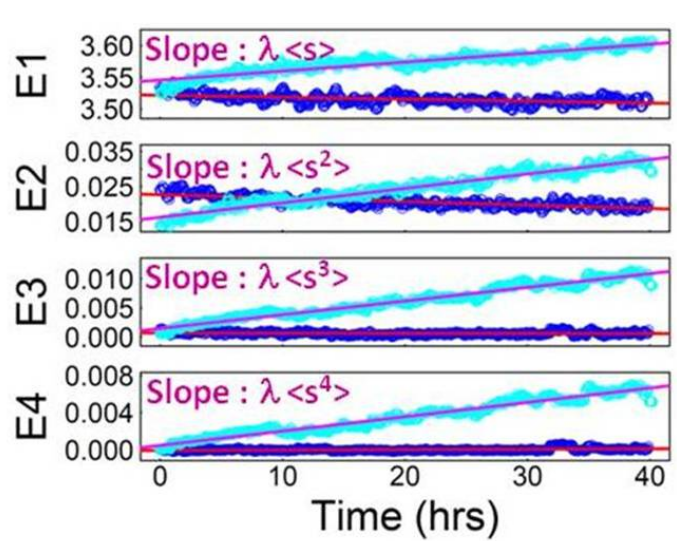
\includegraphics[scale=0.3]{img/supmat_lines.png}
  \end{center}
  \caption{\label{lines}Graphes de $t\mapsto E_n(t)$ pour $n=1,2,3,4$, obtenus dans \cite{rob}, pour les souches WT (en bleu foncé) et \emph{MutH} (en bleu clair). Les droites correspondent aux régressions linéaires effectuées.}
\end{figure}

\begin{figure}[h]
  \begin{center}
    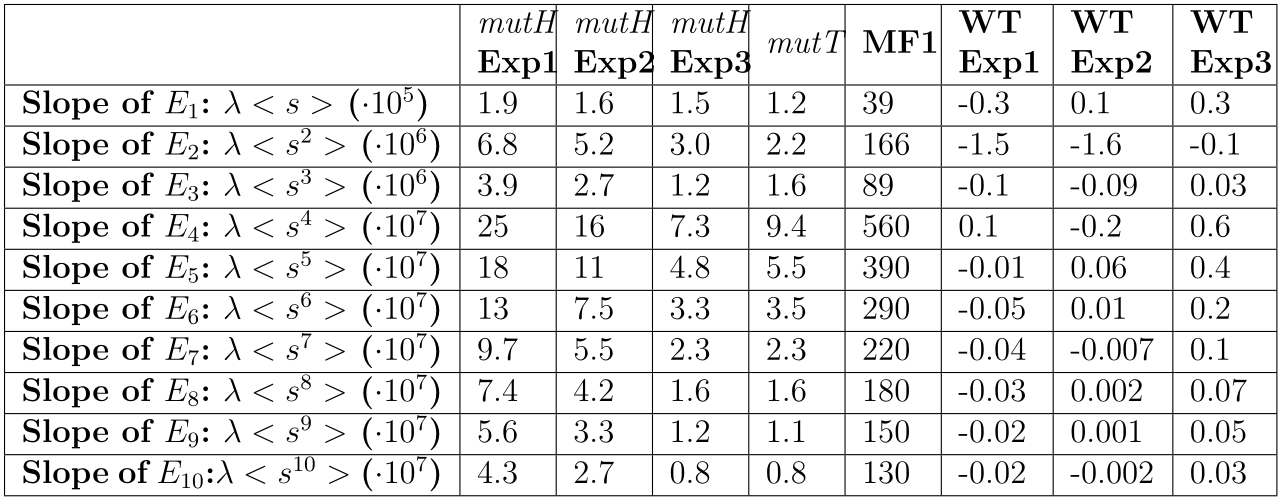
\includegraphics[scale=0.3]{img/supmat_slopes.png}
  \end{center}
  \caption{\label{slopes}Pentes obtenues dans \cite{rob} pour les 10 premiers moments sur les souches \emph{mutH} (trois expériences), \emph{mutT}, \textbf{MF1}, \textbf{WT} (trois expériences).}
\end{figure}

\begin{figure}[h]
  \begin{center}
    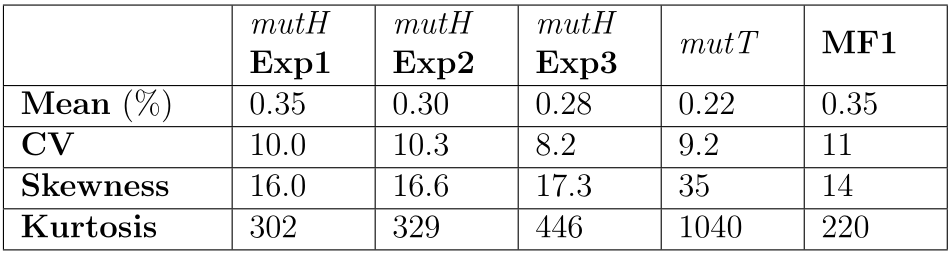
\includegraphics[scale=0.3]{img/supmat_moments.png}
  \end{center}
  \caption{\label{moments}Estimations obtenues dans \cite{rob} de la moyenne, de l'écart-type, du coefficient d'asymétrie et de la kurtosis pour les DFE de trois souches (\emph{mutH}, \emph{mutT}, \textbf{MF1})}
\end{figure}



\paragraph{Traitement initial des données}

Les données obtenues dans l'expérience $\mu$MA sont très bruitées. Nous indiquons ici les transformations effectuées sur ces données afin d'obtenir des résultats corrects:
\begin{itemize}
\item Sélection des cellules qui sont encore vivantes à la $44^e$ heure. Cela se justifie par le fait que les cellules qui croissent très lentement ou qui sont mortes induisent du bruit dans l'estimation de la DFE. Nous avons pu vérifier que le conditionnement effectué (<<~on suppose que la cellule ne meurt pas au cours de l'expérience~>>) n'induit pas de biais majeur dans l'estimation des moments;
\item Pour éviter les erreurs d'analyse d'image, les taux de croissances des lignées ayant un taux de croissance très faible (inférieur à $0.015$) ont été vérifiés visuellement;
\item L'analyse d'image peut créer des valeurs aberrantes. Ces valeurs aberrantes ont été supprimées ainsi: si une valeur au temps $t$ diffère d'au moins $30\%$ simultanément de la médiane des valeurs prises avant le temps $t$, et de la médiane des celles prises après le temps $t$, alors ont supprime cette valeur.
\end{itemize}


\paragraph{Prise en compte du bruit multiplicatif}

Les auteurs de \cite{rob} ont montré que, en supposant que le bruit sur la mesure des taux de croissance est multiplicatif, alors la pente de $E_n(t)$ n'est pas modifiée par le bruit. Un bruit purement multiplicatif n'influence donc pas l'estimation des moments. Plus précisément, notons $W'_{t_i}$ le taux de croissance mesuré au temps $t_i$, et $W_{t_i}$ le taux de croissance réel au temps $t_i$. L'hypothèse du bruit multiplicatif suppose que $W'_{t_i}=W_{t_i}(1+\varepsilon_i)$ où les $\varepsilon_i$, $i\in\En$ sont des variables aléatoires indépendantes, identiquement distribuées, et indépendantes des $W_t$. On a:
\[\ln\Esp{W'_{t_i}}=\ln\pth{\Esp{W_{t_i}}\Esp{1+\varepsilon_i}}=\ln\Esp{W_{t_i}}+\ln\Esp{1+\varepsilon}\]
ce qui fait que l'estimation $E'_n(t)$ que l'on fait de $E_n(t)$ diffère de $E_n(t)$ d'un terme indépendant de $t$. Ainsi, l'ordonnée à l'origine de la droite est modifiée, mais pas sa pente.



\FloatBarrier
\section{Annexe: Vérification\label{ann:verif}}

La figure \ref{fig:iv_verif} montre les graphes des fonctions suivantes, trouvées dans \ref{ss:det_dfe}, pour différentes valeurs de $\xi$:
\begin{align*}
  \ln\abs{\fr u_t(\xi)}&=\ln\abs{\fr u_0(\xi)}+t\times\Re(a_{\xi})\\
  \arg\pth{\fr u_t(\xi)}&=\arg{\fr u_0(\xi)}+t\times\Im(a_{\xi})
\end{align*}

\begin{figure}[h]
  \begin{center}
    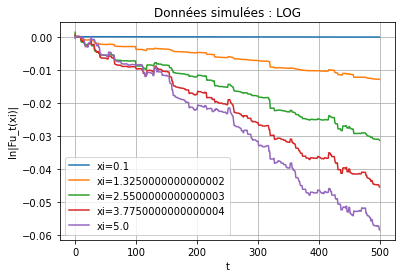
\includegraphics[scale=0.6]{img/iv_verif_pxi.png}
    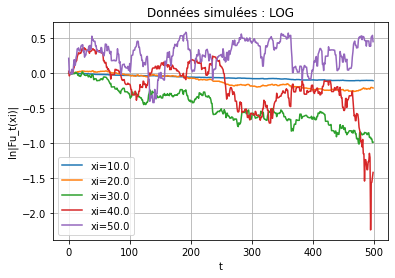
\includegraphics[scale=0.6]{img/iv_verif_grxi.png}
    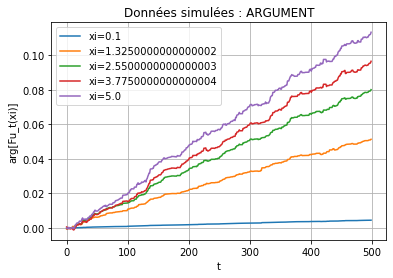
\includegraphics[scale=0.6]{img/iv_verif_pxi_im.png}
  \end{center}
  \caption{\label{fig:iv_verif}Premier graphique: droites dont les pentes doivent donner $a_{\xi}$ (petites valeurs de $\xi$); deuxième graphique: pour de grandes valeurs de $\xi$, on n'obtient pas de droites: cela est peut-être dû à l'overfitting; troisième graphique: droites dont les pentes doivent donner $a_{\xi}$ (petites valeurs de $\xi$).}
\end{figure}




\end{document}
